\graphicspath{{figures/research/}}
\chapter{Background Research}\glsresetall
\label{cha:research}
To be able to further develop on the tracking system presented in the \nameref{ch:intro}, background research and system analysis is necessary. In this chapter, the existing Loligo Systems solution LoliTrack is presented as well as the company it self, together with the an overview of tasks to solved for 3D tracking implementation. A further state of the art solutions is presented in \autoref{ch:analysis}.

\section{Loligo Systems}
Loligo Systems is a company who specialise in aquatic biology research, animal physiology, and  behavioural research equipment. The equipment mainly consist of animal chambers, flumes, sensors, instruments and software for automated oxygen consumption measurements, and equipment for video-based tracking and analysis of animal behaviour. Examples of product are shown in \autoref{fig:loliproducts}.

\begin{figure}[H]
	\centering
	\begin{subfigure}{0.33\textwidth}
		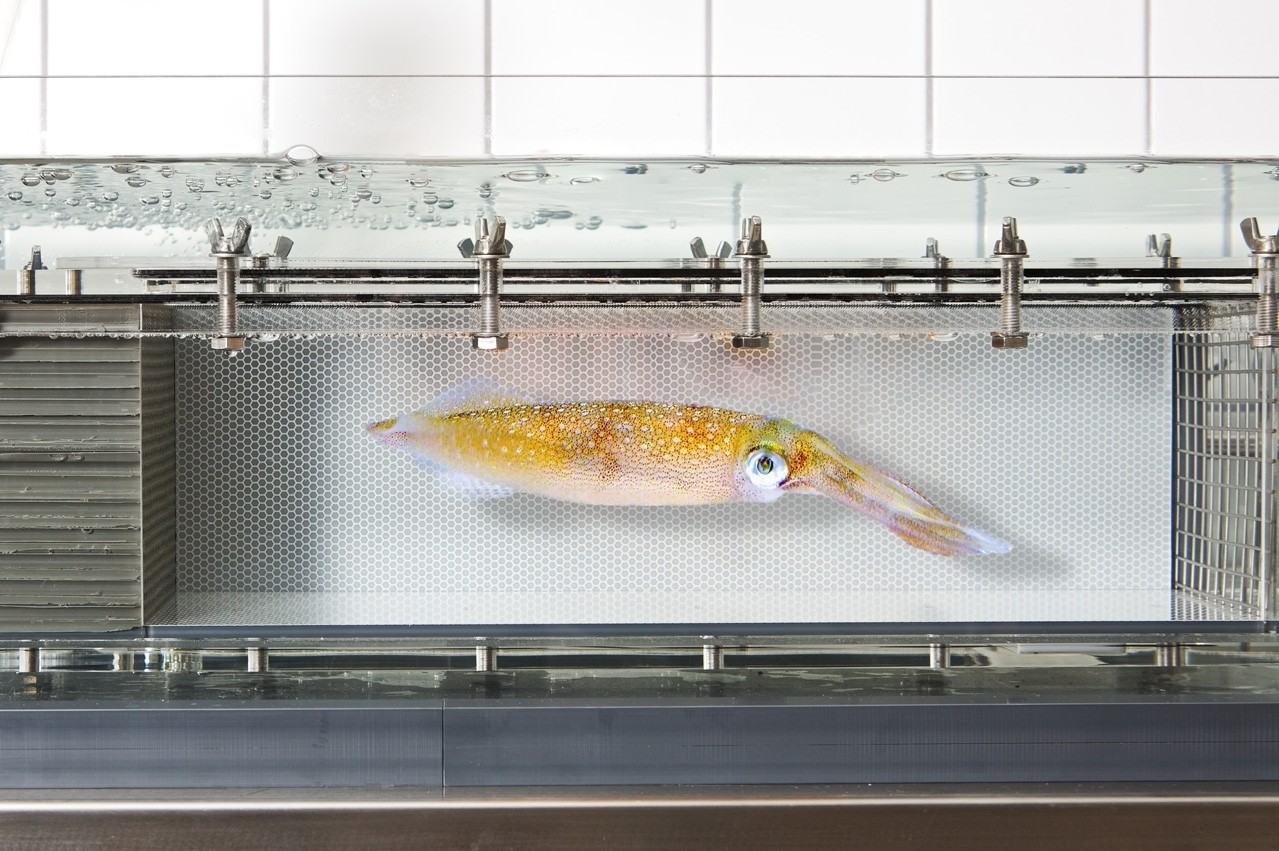
\includegraphics[width=\textwidth]{swimming-performance}
		\caption{Swimming chamber to measure swimming performance.}
	\end{subfigure}
	\begin{subfigure}{0.33\textwidth}
		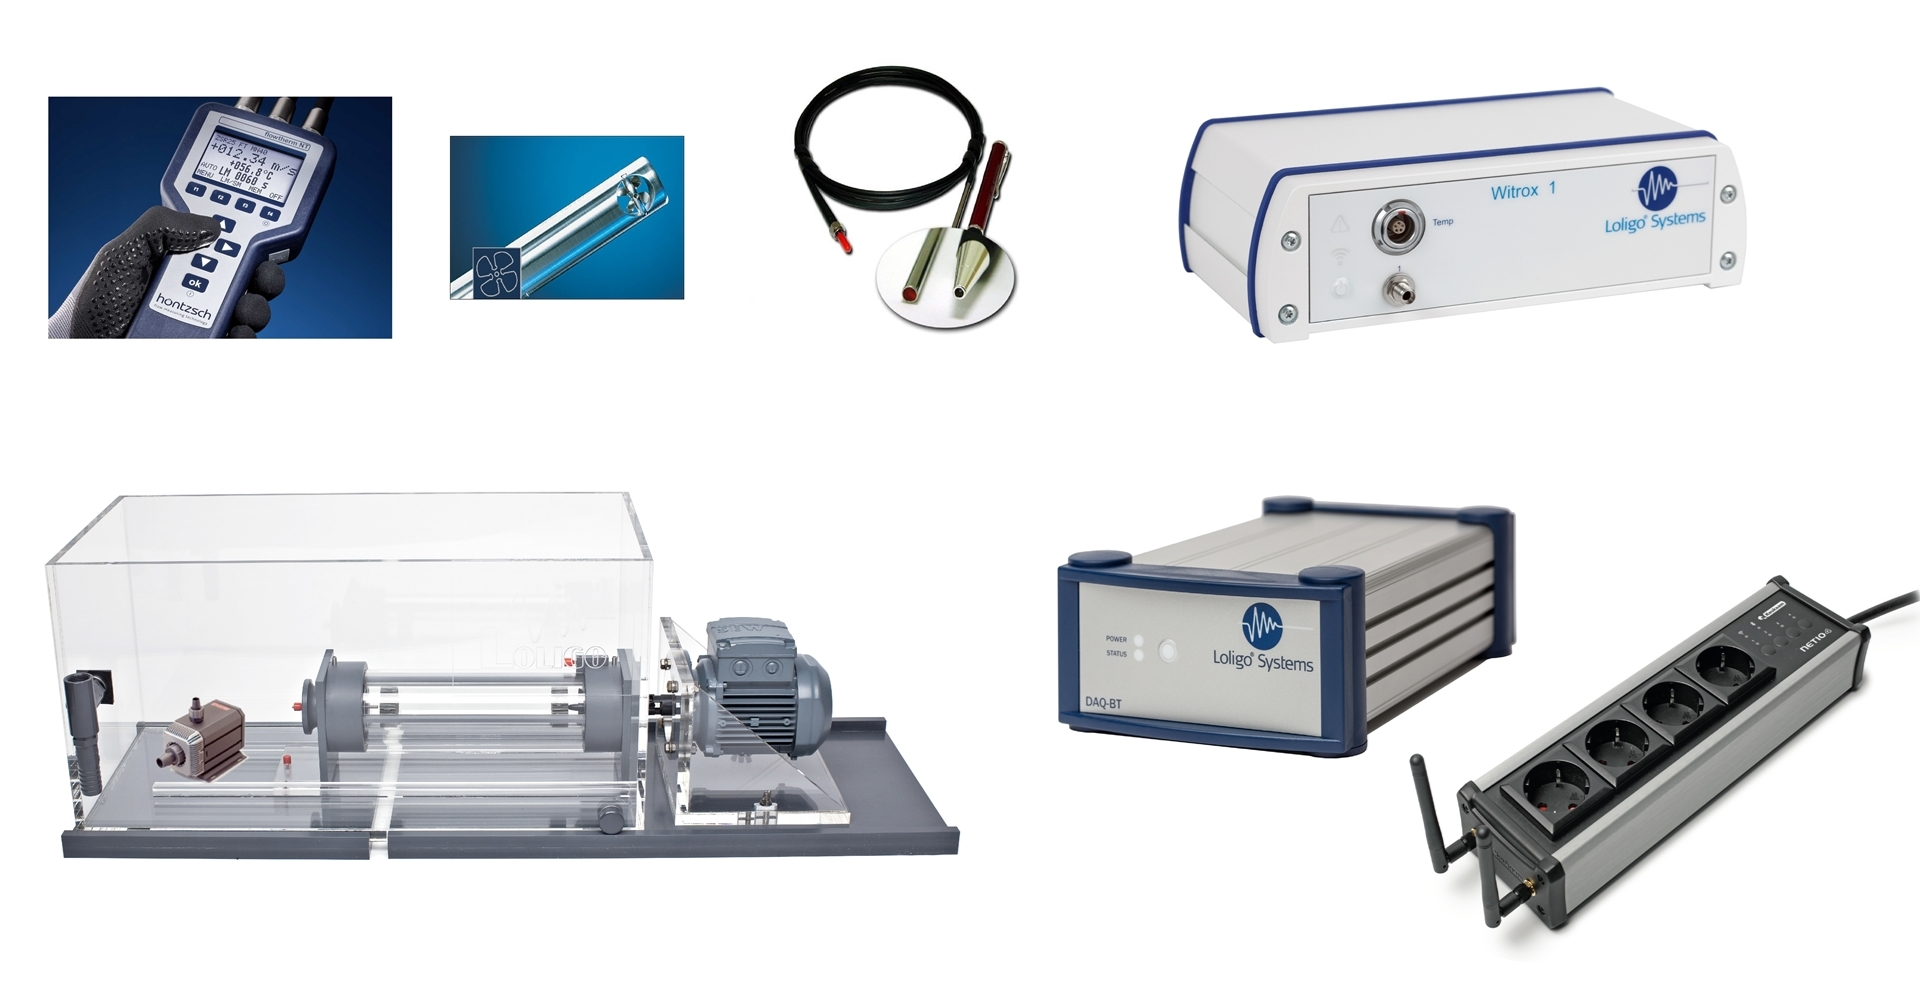
\includegraphics[width=\textwidth]{swimming-respirometry}
		\caption{Swimming chamber fish respirometry. Full package for testing.}
	\end{subfigure}
	\begin{subfigure}{0.32\textwidth}
		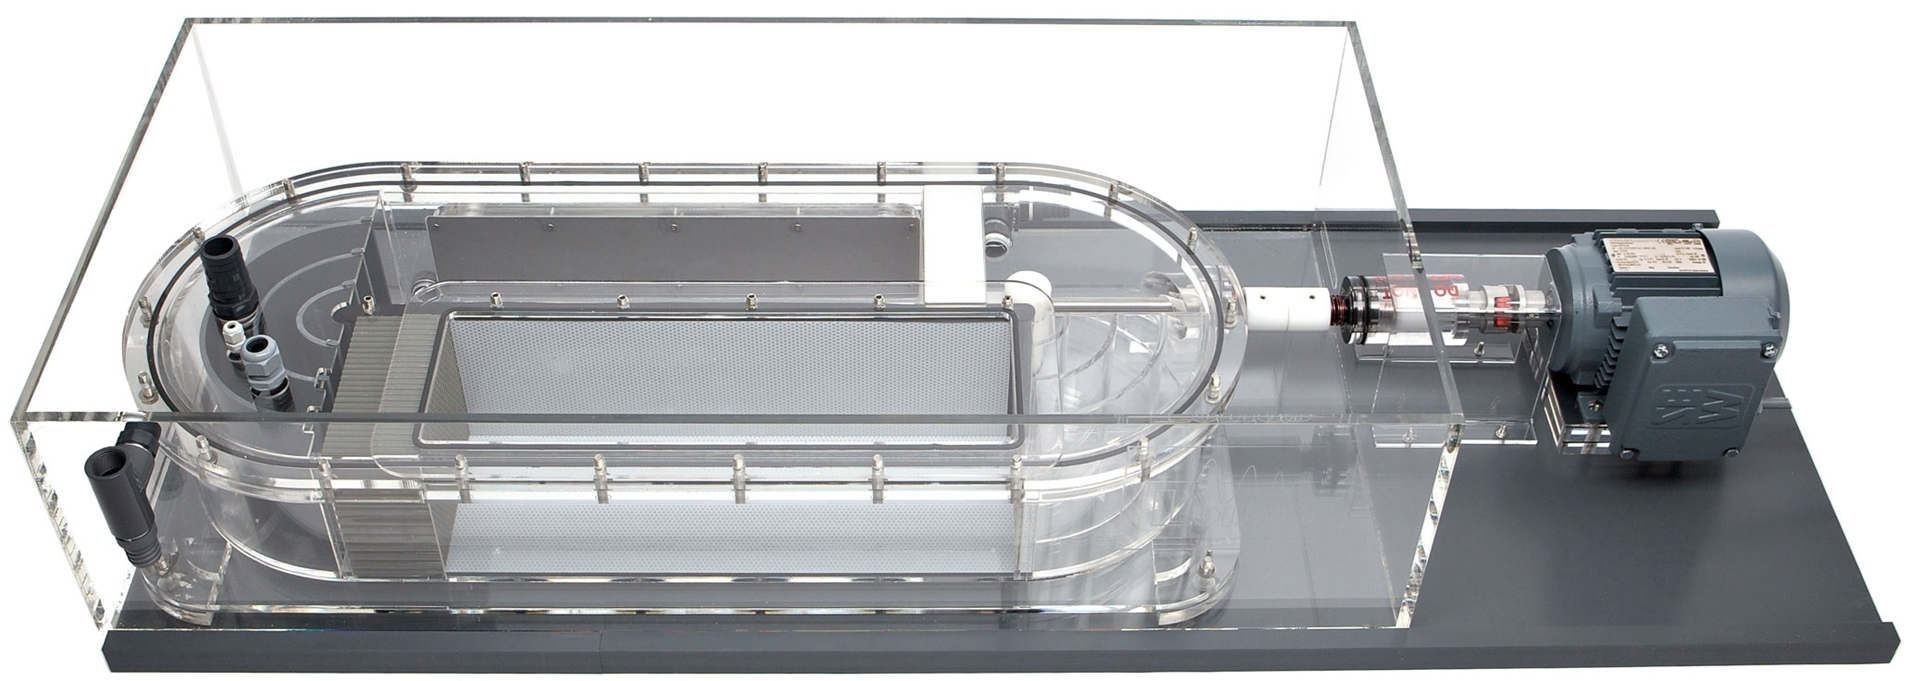
\includegraphics[width=\textwidth]{swim-tunnel-respirometer}
		\caption{Swimming tunnel to test swimming performance under different circumstances.}
	\end{subfigure}
\caption{Overview of a few hardware solution products sold by Loligo Systems}
\label{fig:loliproducts}
\end{figure}

\subsection{LoliTrack}
One of the product developed and sold by Loligo Systems, is the software solution LoliTrack. This is a 2 dimensional tracking solution, which is claimed to be able to track up to 24 objects inside a single arena and able to handle occlusions. The system is made to be used with any camera solution and is contrast based using contrasted background. The software produces an x- and a y-coordinate pair assigned to the centre point of the object tracked. From this data several parameters are produced, consisting of; active/inactive time, velocity, acceleration, direction of movement, direction of orientation, and more. Example images from Loligo's website are shown in \autoref{fig:lolitrack_examples}.

\begin{figure}[H]
	\centering
	\begin{subfigure}{0.45\textwidth}
		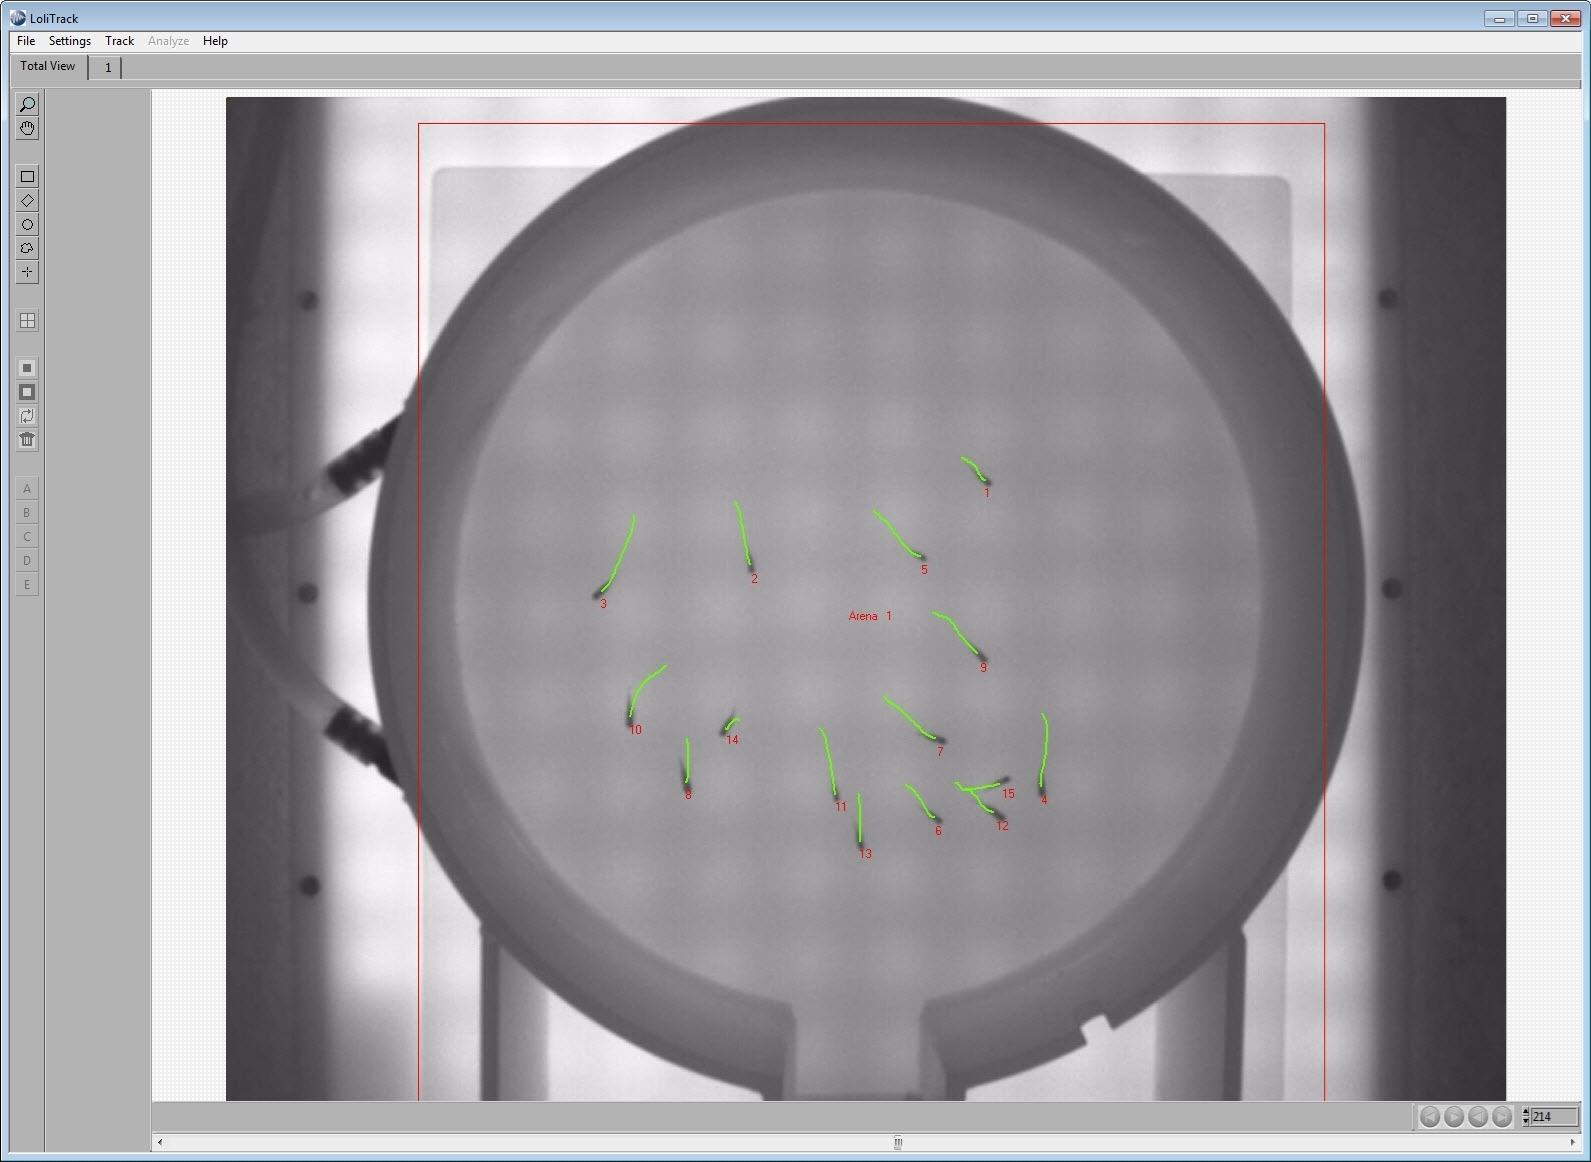
\includegraphics[width=\textwidth]{lolitrack-fish}
		\caption{LoliTrack working on one arena with multiple objects of Zebra Fish}
	\end{subfigure}
	\begin{subfigure}{0.45\textwidth}
		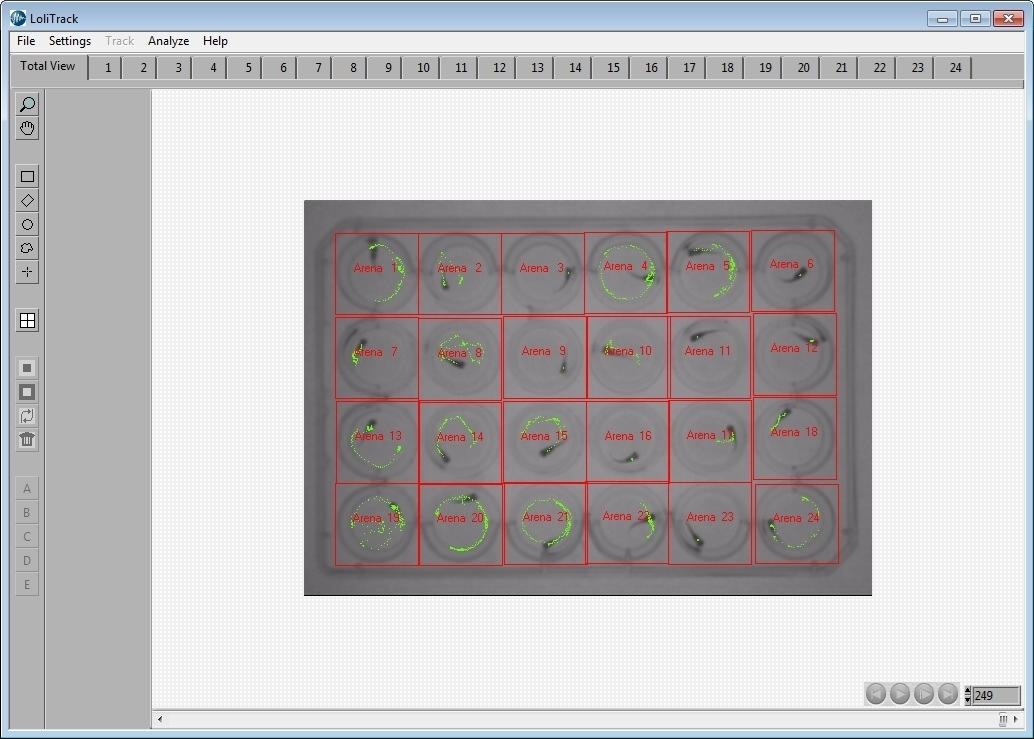
\includegraphics[width=\textwidth]{lolitrack-mult-arena}
		\caption{LoliTrack working on multiple arenas with a single object in each arena}
	\end{subfigure}
	\caption{Overview of a few LoliTrack examples}
	\label{fig:lolitrack_examples}
\end{figure}

According to Loligo Systems the detection and tracking is done in six steps:

\begin{enumerate}
	\item RGB to binary image conversion using the high contrast difference of the fish and background.
	\item Noise reduction using dilation.
	\item Blob identification and extraction.
	\item Pixels in blobs are given a value between $1$ and $3$ dependent on distance to blob centre.
	\item Every blob is fitted with a two-dimensional Gaussian distribution to the values of the pixel values given.
	\item Step 1-4 is repeated for every frame. Afterwards expectations maximisation is used dependent on the previous frames.
\end{enumerate}

\subsection{New LoliTrack Setup}
IDS NIR cameras - NIR backlit aquarium - high contrast between fish an background - undetectable water

\section{Fish Detection}
In computer vision multiple approaches to detect an object exist. The suitable approach depends on the application area and is done both using regular machine learning but also deep learning.

In every scenario, a detection application is an image processing task aimed at detecting the desired objects in an image while refraining from creating false positives. The output should the be at least x-, y-coordinates and a frame number for every detection.

Existing solutions of detection are presented in \autoref{ch:analysis}. 

\section{Fish Tracking}
When tracking in two dimensional space, a simple solution is generating tracks by associating the detections made in each frame and minimising the travel distance of the fish in the successive frames.

With multiple fish in the scene, each fish needs to be tracked separately. Having multiple fish can result in occlusions and missed detections, which can lead to faulty tracking because of swapped ID between fish or missing tracks for a period.

Suggested state of the art solutions to tracking fish are presented in \autoref{ch:analysis}.